% !TEX encoding = UTF-8 Unicode
% $Header: /cvsroot/latex-beamer/latex-beamer/solutions/conference-talks/conference-ornate-20min.en.tex,v 1.6 2004/10/07 20:53:08 tantau Exp $

\documentclass{beamer}

\mode<presentation>
{
  \usetheme{Warsaw}
  % or ...

  \setbeamercovered{invisible}
  % or whatever (possibly just delete it)
  
  \setbeamertemplate{navigation symbols}{}
  
  \newcommand*\oldmacro{}%
  \let\oldmacro\insertshorttitle%
  \renewcommand*\insertshorttitle{%
    \oldmacro\hfill%
    \insertframenumber\,/\,\inserttotalframenumber}
}

\usepackage[utf8]{inputenc}
% or whatever

\usepackage{times}
\usepackage{multirow}
\usepackage[T1]{fontenc}
\usepackage[french]{babel}
\usepackage{graphicx}

\usepackage{eso-pic}
\usepackage{color}
\usepackage{tikz}
\usepackage{wasysym}

% Or whatever. Note that the encoding and the font should match. If T1
% does not look nice, try deleting the line with the fontenc.

\title[Prologin in Black]
{}

\titlegraphic{\raisebox{2em}{}}

\author[Prologin]
{
\includegraphics{../prologin2018}}

\date
{}

\begin{document}

\begin{frame}
    \centering 
\includegraphics[width=0.9\linewidth]{../prologin2018}
    \vspace{1.5cm}
    \textbf{Prologin in Black}

    \vspace{0.5cm}
    \footnotesize{\color{red}TOP SECRET//SI//ORCON//NOFORN}
\end{frame}

\begin{frame}
    \frametitle{L'organisation PiB}
    \begin{itemize}
        \item Créée en 1965 sur un consensus international
        \item Surveille et repousse les tentatives d'invasion alien
        \item Inconnue de tous... Jusqu'à \textbf{aujourd'hui}
    \end{itemize}
\end{frame}

\begin{frame}
    \frametitle{Contexte intergalactique}
    FIXME
    \begin{itemize}
        \item Détection d'un groupe extra-terrestre
        \item Justification invasion
        \item Phase de repérage
    \end{itemize}
\end{frame}

\begin{frame}
    \frametitle{Déroulement de la mission}
    \begin{center}
        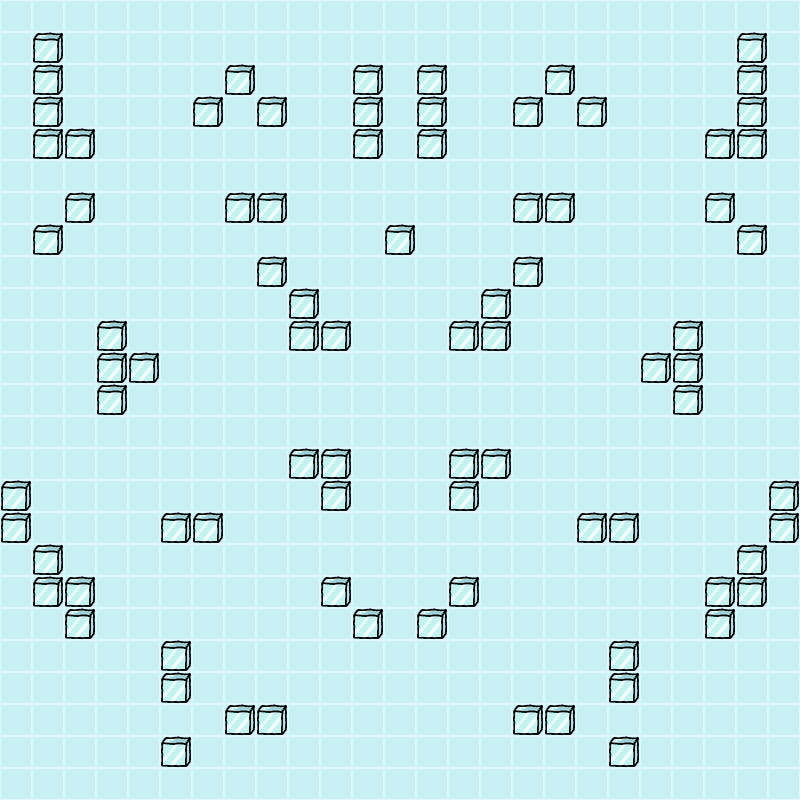
\includegraphics[width=0.65\textwidth]{../img/map}
    \end{center}
\end{frame}

\begin{frame}
    \frametitle{Nos agents de terrain}
    \begin{center}
        
\includegraphics[width=0.7\textwidth]{../logofinale}
    \end{center}
\end{frame}

\begin{frame}
    \frametitle{Contrôle à distance}
    \begin{itemize}
        \item Déplacement simple
        \item Glissade
        \item Pousser
    \end{itemize}
\end{frame}

\begin{frame}
    \frametitle{Les aliens}
\end{frame}

\begin{frame}
    \frametitle{Questions}
    Posez vos questions sur le brief de mission !
\end{frame}

\begin{frame}
    \frametitle{Tournois intermédiaires}
    \begin{itemize}
        \item Samedi 15~h~42 (tournoi test)
        \item Samedi 17~h~42
        \item Samedi 23~h~42
        \item Dimanche 5~h~42
        \item Dimanche 11~h~42
        \item Dimanche 17~h~42
        \item Lundi 00~h~42 (tournoi final)
    \end{itemize}
\end{frame}

\begin{frame}
    \frametitle{Fin}
    Importance vestimentaire...
\end{frame}

\end{document}
